\chapter{Аналитическая часть}

	В данном разделе рассмотрены физические основы преломления, существующие алгоритмы построения реалистических изображений и способы хранение трехмерных объектов. Обосновывается выбор алгоритмов и форматов 3д объектов для реализации поставленной задачи. 

	\section{Физическая модель оптических линз}
	Оптическая линза (далее просто линза) - деталь из прозрачного однородного материала, имеющая две преломляющие поверхности, например, обе сферические или же одну плоскую, другую - сферическую.
	Для объяснения физики преломления света при прохождении через оптические линзы, необходимо ввести следующие понятия \cite{1988phs}:
	\begin{itemize}
	\item[--] свет - электромагнитное излучение, распространяемое в виде волны;
	\item[--] поляризованный свет — это свет, в котором направление колебаний вектора напряженности электрического поля упорядочено;
	\item[--] неполяризованный свет - естественный свет, в котором вектор напряженности электрического поля может с равной вероятностью иметь любое направление колебаний в плоскости, перпендикулярной направлению распространения света;
	\item[--] световой луч (луч) -- линия, вдоль которой распространяется световая волна;
	\item[--] фаза луча -- состояние световой волны в момент времени (функция координат и времени);
	\item[--] длина волны -- расстояние между двумя ближайшими друг к другу точками в пространстве, в которых колебания происходят в одинаковой фазе;
	\item[--] абсолютный коэффициент преломления -- безразмерная физическая величина, характеризующая различие фазовых скоростей света в двух средах;
	\item[--] относительный показатель преломления -- безразмерная величина, показывающая отношение абсолютных показателей преломления двух сред.
	\item[--] интенсивность луча -- энергия, переносимая лучом в заданном направлении (от нее зависит яркость излучения).
	\end{itemize}
	
	На рисунке \ref{img/refraction} представлено поведение луча на границе двух сред с разными коэффициентами преломления. Луч, падающий на границу двух веществ, лежит в плоскости чертежа и задан вектором ${k}$, а нормаль к поверхности раздела задана вектором ${n}$. Линия пересечения плоскости падения луча и границы раздела двух сред задана осью $x$, ось $y$ направлена перпендикулярно к плоскости раздела сред. Траектория луча в таком случае представлена на рисунке \ref{img/refraction}.
	
	\begin{figure}[H]
		\center{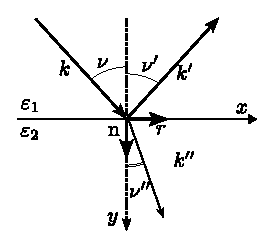
\includegraphics[width=\textwidth, height=50mm, width=170mm, keepaspectratio]{img/refraction.eps}}
		\caption{Траектория луча на границе двух сред}
		\label{img/refraction}
	\end{figure}
	
		Преломленный луч лежит в одной плоскости с падающим лучом и нормалью, востановленной в точке падения. Отношение синуса угла падения к синусу угла преломления есть постоянная величина для заданных веществ.\cite{savelev} При этом углы преломления и отражения задаются уравнениями \ref{eq/refraction_angle} и \ref{eq/reflection_angle} соответвенно.
\begin{equation}
\label{eq/refraction_angle}
n_1 \sin \nu = n_2 \sin \nu ''
\end{equation}
\begin{equation}
\label{eq/reflection_angle}
\nu = \nu'
\end{equation}

Существует два основных коэффициента отражения: для света с параллельной поляризацией ($R_p$) и для света с перпендикулярной поляризацией ($R_s$):
\begin{eqnarray}
\label{eq/FrenelPerp}
R_s = \left( \frac{n_1\cos(\theta_1) - n_2\cos(\theta_2)}{n_1 \cos(\theta_1) + n_2 \cos(\theta_2)} \right)^2\\
\label{eq/FrenelParall}
R_p = \left( \frac{n_2\cos(\theta_1) - n_1\cos(\theta_2)}{n_2 \cos(\theta_1) + n_1 \cos(\theta_2)} \right)^2,
\end{eqnarray}
где:
\begin{itemize}
\item[--] $n_1$ 	и $т_2$ -- показатели преломления первой и второй среды;
\item[--] $\theta_1$ -- угол падения луча на поверхность раздела сред;
\item[--] $\theta_2$ -- угол преломления, который вычисляется по закону \ref{eq/refraction_angle}.
\end{itemize}

Для неполяризованного света коэффициент отражения рас	считывается по формуле:
\begin{equation}
R = \frac{R_s + R_p}{2}
\end{equation}

Коэффициент преломления будет рассчитываться по формуле:
\begin{equation}
T = 1 - R
\end{equation}

При прохождение луча через линзу может наблюдаться явление дисперсии - расхождение световых лучей разного цвета.
    \section{Формализация задачи}
    Формализованная задача представлена на рисунке
    
    	\begin{figure}[H]
		\center{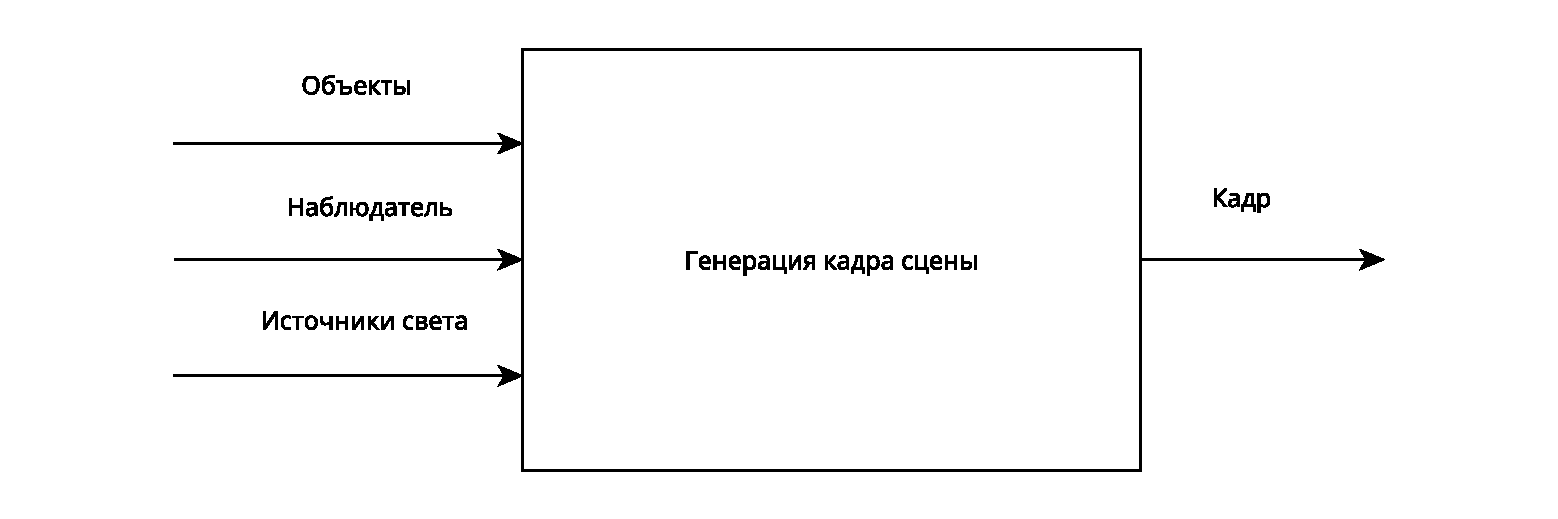
\includegraphics[width=\textwidth, height=1700mm, width=170mm, keepaspectratio]{img/idef0.eps}}
		\caption{Формализованная задача с учетом выбранных алгоритмов}
		\label{img/idef0}
	\end{figure}
	
	\section{Формализация объектов сцены}
	На сцене могут присутствовать следующие типы объектов:
	\begin{itemize}
	\item[--] Сферы с параметрами радиуса, прозрачности, коэффициентом преломления, цветом, уветом излучения и интенсивностью излучения (при излучении света, лучи направлятся в направлении нормали к поверхности сферы);
	\item[--] Линзы с параметрами радиуса, радиуса кривизны, прозрачности, цвета и коэффициента преломления;
	\item[--] Наблюдатель (задается положением, напрвлением зрения и углом обзора);
	\item[--] Полигоны (задаются тремя точками и цветом);
	\end{itemize}
	
	\section{Модель освещения}
	Модель освещения определяет интенсивность освещения $I$ в каждой точке. Наиболее распространенными моделями освеения являются глобальная и лоакльная \cite{leb2011}.
	
	В локальной модели освещения каждый объект рассматривается по отдельности, без учета взаимодействия с другими объектами. Глобальная модель освещения учитывает взаимное расположение объектов. Поскольку для корректного отображения преломления света через линзы необходимо учитывать их взаимное расположение, будет использоваться глобальная модель освещения.
	
	В глобальной модели освещения для каждой точки $P$ пространства сцены интенсивность освещения $I$ будет рассчитываться из 4 состовляющих:
	\begin{itemize}
		\item[--] фоновое освещение, существующее в каждой точке пространства сцены, не зависящее от источников света и координаты точки.
		\item[--] рассеянный свет, распространяющийся равномерно во все стороны, при попадании луча на поверхность объекта, зависящий от ориентации поверхности (нормали $N$ к поверхности в точке), направления на источник света $L$ и интенсивности источника;
		\item[--] зеркальная составляющая, зависящая от зеркальности поверхности и от того, насколько близки направления на наблюдателя и отраженного луча;
		\item[--] преломленная составляющая, зависящая от интенсивности преломленного луча.
	\end{itemize}
	
	Поскольку в задача работы состоит в отображении преломления через лензы, предлагается упростить модель освещения, не учитывая рассеянный свет. В таком случае итоговая составляющая будет рассчитываться по формуле:
	\begin{equation}
	I = k_{\alpha}I_{\alpha} + \sum_j I_j(\overline{N} \cdot \overline{L_j}) + k_{r} I_{r} + k_s I_s
	\end{equation}
	
	где:
	\begin{itemize}
	\item[] $k_{\alpha}$ -- коэффициент фонового освещения;
	\item[] $k_{r}$ -- коэффициент пропускания;
	\item[] $k_s$ -- коэффициент отражения;
	\item[] $I_j$ -- интенсивность j-го источника света;
	\item[] $I_r$ -- интенсивность преломленного луча;
	\item[] $I_s$ -- интенсивность отраженного луча;
	\item[] $\overline{N}$ -- нормаль к поверхности в точке;
	\item[] $\overline{L_j}$ -- вектор, направленный к j-му источнику.
	\end{itemize}
	
	\subsection{Метод фотонных карт}
	Алгоритм создания изображения состоит из трех шагов: на первом шаге испускаются прямые лучи из источников света, распространяются по сцене и формируют распределение фотонов на диффузных поверхностях сцены; на втором шаге на основе полученного распределения фотонов формируются фотонные карты для объектов сцены; на последнем шаге из камеры испускаются обратные лучи и ищется их пересечение с фотонными картами\cite{zhdanov2020}. В точках пересечения с фотонными картами происходит перерасчет светового потока, переносимого фотоном, в яркость вторичного излучения, наблюдаемую в данном направлении:
	     \begin{figure}[H]
		\center{\includegraphics[width=\textwidth, height=70mm, width=170mm, keepaspectratio]{img/photons.png}}
		\caption{Сбор распределения яркости с фотонов при трассировке обратного луча}
		\label{img/photons}
	\end{figure}
	
		\subsection{Простроение освещения с помощью трассировки лучей}
	В алгоритме используется модификация алгоритма, описанного в пункте 1.5.4. Для расчета непрямого освещения для каждой точки дифуззной поверхности при пересечении с лучом трассировки испускается заданное число случайных лучей. После чего они трассируются и на основе их увета формируется непрямое освещение. Такой метод очень трудозатратный, т.к. для количество лучей трассировки резко возрастает.
	

    
    \section{Алгоритмы удаления невидимых поверхностей}

		Удаление невидимых линий и поверхностей заключается в определении тех частей объектов, которые видимы или невидимы для наблюдателя из определенной точки пространства. Эта задача может решаться в двух пространствах:

\begin{itemize}
\item Объектное пространство -- используется физическая система координат, в которой описаны объекты сцены, обеспечивает высокую точность изображения;
\item Пространство изображения -- используется система координат экрана, на котором визуализируется полученное изображение, точность вычислений ограничена разрешающей способностью экрана. 
\end{itemize}
	
	Самыми распространенными алгормами, решающими задачу являются: алгоритм Робертса, z-буффера, трассировки лучей.
        
        \subsection{Алгоритм Робертса}
        Алгоритм Робертса — это один из первых методов для удаления невидимых линий, работающий в объектном пространстве. Он удаляет те ребра и грани, которые скрыты самим объектом\cite{capko2010}. Затем оставшиеся видимые ребра сравниваются с другими объектами для определения, какие их части могут быть скрыты.

	Трудоемкость алгоритма возрастает пропорционально квадрату количества объектов. Он подходит только для работы с выпуклыми телами, а невыпуклые объекты необходимо разбивать на выпуклые части. Поздние версии алгоритма используют предварительную сортировку для повышения эффективности.            

        \subsection{Алгоритм Z--буфера}
        Алгоритм z-буфера — это один из простейших методов удаления невидимых поверхностей в 3D-графике, предложенный Кэтмулом\cite{zbuf2015}. Он работает в пространстве изображения, используя отдельный буфер для хранения глубины каждого видимого пикселя. При отрисовке нового пикселя его глубина сравнивается с той, что уже записана в буфер. Если новый пиксель ближе, он заменяет предыдущий в буфере кадра, и z-буфер обновляется его глубиной. Алгоритм прост, не требует сортировки по глубине, но требует большого объема памяти и может быть менее эффективным при прозрачности или антиалиасинге.

	Пример работы алгоритма, использующего z--буфер, представлен на рисунке \ref{img/z_buffer}.
	
        	\begin{figure}[H]
		\center{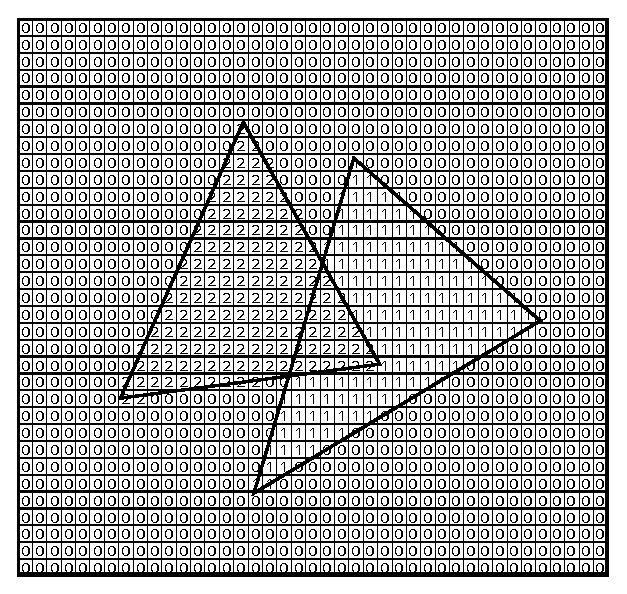
\includegraphics[width=\textwidth, height=130mm, width=170mm, keepaspectratio]{img/z_buffer.eps}}
		\caption{Пример работы алгоритма Z--буфера}
		\label{img/z_buffer}
	\end{figure}
	
		\subsection{Алгоритм Варнока}
        
        Алгоритм Варнока основан на принципе когерентности изображения, при котором большие однородные области требуют меньше усилий для обработки\cite{varnok2017}. Он работает в пространстве изображения и разбивает его на подокна, чтобы определить, простое ли их содержимое. Если содержимое сложное, окно делится дальше, пока не достигнет уровня пиксела. Пример работы алгоритма представлен на рисунке \ref{img/Varnok}.
        
	\begin{figure}[H]
		\center{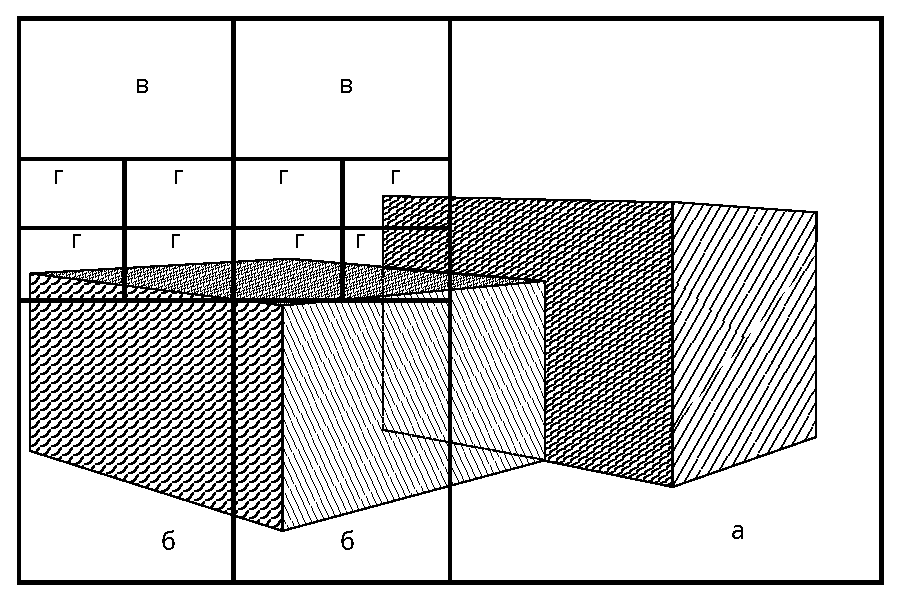
\includegraphics[width=\textwidth, height=70mm, width=170mm, keepaspectratio]{img/Varnok.eps}}
		\caption{Пример работы алгоритма Варнока}
		\label{img/Varnok}
	\end{figure}
        	

Основная идея алгоритма — сосредотачивать вычислительные ресурсы на сложных частях сцены, игнорируя простые области. Метод эффективен для удаления невидимых линий и поверхностей.



                       
        \subsection{Алгоритм обратной трассировки лучей}
        Алгоритм обратной трассировки лучей заключается в том, что для определения видимых поверхностей сцены лучи отправляются от наблюдателя к объекту\cite{backray2006}. Трассировка каждого луча позволяет выяснить, какие объекты сцены пересекаются с данным лучом, учесть преломления, отражения и прохождение сквозь объекты. Пересечения объектов с лучом упорядочиваются по глубине, и ближайшее пересечение указывает на видимую поверхность для каждого пикселя. Пример трассировки лучей представлен на рисунке \ref{img/forward_tras}.
     
     \begin{figure}[H]
		\center{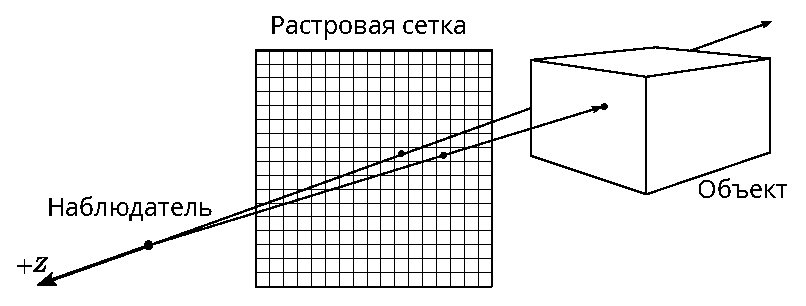
\includegraphics[width=\textwidth, height=70mm, width=170mm, keepaspectratio]{img/forward_tras.eps}}
		\caption{Обратная трассировка лучей}
		\label{img/forward_tras}
	\end{figure}

Основной сложностью алгоритма является определение точек пересечения луча с объектами сцены. Для оптимизации вычислений вводятся габаритные тесты с объемными оболочками (сферами или параллелепипедами) для исключения объектов, с которыми луч не пересекается.

Алгоритм эффективен, если пересечения вычисляются быстро и точно, что существенно влияет на общую производительность. 
                

    
    \section{Способы хранения трехмерных объектов}
   	
   	Классификацию форматов трехмерных бъектов можно провести по 2 параметрам -- это способ описания их геометрии и способ описания их внешнего вида\cite{3f_content_overview}.
   	
   	\subsection{Геометрические параметры 3д объектов}
   		
   	Геометрия моделей часто задаются набором трехмерных точек. Поверхность в таком случае сохраняется ввиде ряда полигонов, которые создаются путем индексации этих вершин. В некоторых форматах используются ребра из 2 вершин. При использовании полигональных моделей для отрисовки круглых объектов можно использовать интерполирование нормалей к каждой грани. При этом существует много вариаций методов интерполирования, наиболее простым из которых является усреднение нормалей, сходящихся в одной вершине, и назначение результата этой вершине. Такой способ хранения 3д объектов достаточен для визуализации 3д контента, где точное определение геометрических свойств не требуется.
   	
   	Для объектов, форму которых можно задать геометрическими примитивами, удобно использовать аналитический способ хранения.
   	   	
   	Другим способом создания 3д моделей является конструктивная твердотельная геометрия. Этот метод использует набор логических операций над геометрическими примитивами. Преимуществом такого метода является точное описание формы объекта, если его так или иначе можно представить набором используемых примитивов, а так же возможность изменить модель на любом этапе ее создания. Данный метод широко используется в САПР.
        
        
    \section{Вывод}

	После оценки вышеизложенных алгоритмов сделан вывод, что для этой работы наиболее подходящим алгоритмом будет алгоритм обратной трассировки лучей, т.к. он позволяет корректно  отобразить симулируемые физические явления, при этом обеспечивая достаточную производительность.
	
Для глобального освещения будет использоваться метод фотонных карт, поскольку он предоставляет возможность моделировать сложные эффекты освещения, такие как мягкие тени, многоступенчатое отражение света и дисперсия, с приемлемым балансом между качеством и производительностью.

	Для хранения линз и сфер будет использоваться аналитический метод(линзы задаются как пересечение двух сфер).